\newpage
\counterwithin{figure}{subsection}
\section{Forward Converter}
\subsection{General Structure}

Forward converter is basically derived from the buck converter. We are going to observe the relationship in the derivation phase. Forward converter is isolated as we know, and it uses transformer as its regular use. Transformer transfers the power to the secondary side and it does not store energy in between. In forward converter, it is important to take the magnetizing current into account.

In Figure \ref{ForwardTopology}, the forward converter topology can be observed. This is the most simple model.

\begin{center}
\begin{figure}[H]
\centering
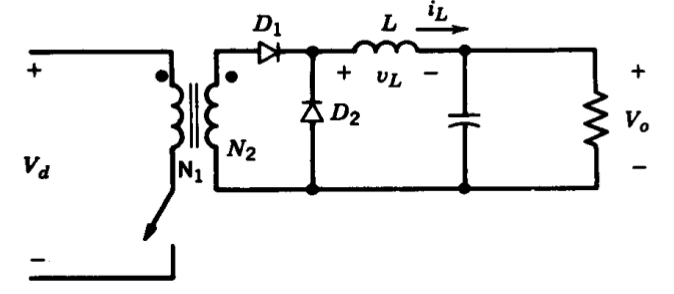
\includegraphics [width= 12 cm ]{forward.png}
\caption{Forward Converter Topology}
\label{ForwardTopology}
\end{figure}
\end{center}

Assume the transformer is ideal for now to obtain the transfer function of the topology. \\During the ON state of the switch, $D_{1}$ is conducting and $D_{2}$ is reverse biased. Therefore, the inductor voltage can be written down as $$V_{L} = \frac{N_2}{N_1}V_{d} - V_{o}$$

Let us examine now the OFF state of the switch. $D_{1}$ is now reverse biased on $D_{2}$ forms a free-wheeling path for the inductor. Load is fed by the stored energy in the inductor and the capacitor. Inductor voltage is easy to obtain and is as follows.$$V_{L} = - V_{o}$$

Discussion so far end with applying the voltage-seconds rule for the inductor and this yields the transfer function of the forward converter topology as 
\begin{equation}
    \frac{V_o}{V_d} = \frac{N_2}{N_1}D
\end{equation}
However, a question might arise rightfully at this point: how does this topology deal with the magnetizing current? During the OFF state, $L_m$ has no path to discharge and it seems to be charged again and again during ON state. This situation ends up saturating the core and threatens the proper operation of the converter. \\
A variety of solutions for this problem are available. A snubber circuitry connected in parallel to the primary winding, a two switch topology are among them. A more practical and wide-spread application ,however, is adding a third reset winding. The resultant topology can be seen in Figure \ref{PracticalForward}.

\begin{center}
\begin{figure}[H]
\centering
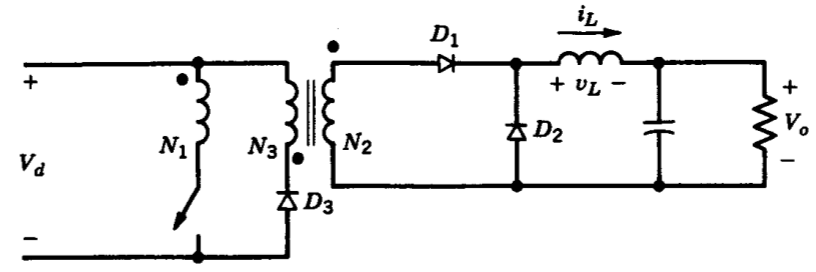
\includegraphics [width= 12 cm ]{practical_forward.png}
\caption{Practical Forward Converter Topology}
\label{PracticalForward}
\end{figure}
\end{center}

In this topology, the third winding namely $N_3$ is in use in order to reset the winding so that the core does not saturate. As its nature opposes, the forward converter has limitations itself. One and the most important thing is that $D_max$ namely maximum duty cycle is limited to the following equation

\begin{equation}
    D_{max} = \dfrac{1}{1 + N_3/N_1}
\end{equation}

In most of the cases, $N_1 = N_3$ is taken to simplify the structure and the organization. We followed the same approach in our solutions.
